\documentclass[a4paper,12pt]{article}
%\usepackage[pdftex]{graphicx}
\usepackage[xetex]{graphicx}
%\usepackage{graphviz}
\usepackage{amssymb}
\usepackage{amsmath}
\usepackage{moreverb}
\usepackage{fancyvrb}
%\usepackage[utf8]{inputenc}
\usepackage{fontspec}
\usepackage[strict]{changepage}
\begin{document}

\title{Formal Methods Homework 2011\\
Solar Heating System}
\author{Lyudmil Angelov\\
Davide Leonarduzzi\\
Camillo Lugaresi}
\date{2011/06/17}
\maketitle

\section{System description}

We have modeled the solar water heating system for a house. Our modeling approach was aimed at enabling the description - and, hopefully, the verification - of the overall behavior of the system operating within its environment: thus, while employing some necessary simplifications, we have striven to model the key aspects of the physical behavior of the plant, of the logical behavior of the controlling software, and even aspects of human behavior (namely, that of the maintainer), imposing appropriate requirements on each so that their interaction results in the desired operation of the complete system.

Modeling the dynamic behaviour of the hydraulic and thermal parts of the system in a time-continuous form would be difficult in TRIO; therefore, the first simplification introduced was to model it as a time-discrete system. It is implied that the scale of the time units should be sufficiently small for the time-discrete approximation to be applicable.

We strove to minimize the number of axioms used to specify the desired behavior, avoiding redundancy. Some significant properties of the system are not included as axioms in the trio specification, but are in fact theorems that should be verifiable from them.

\pagebreak
\subsection{Structure}

\begin{figure}
\centering
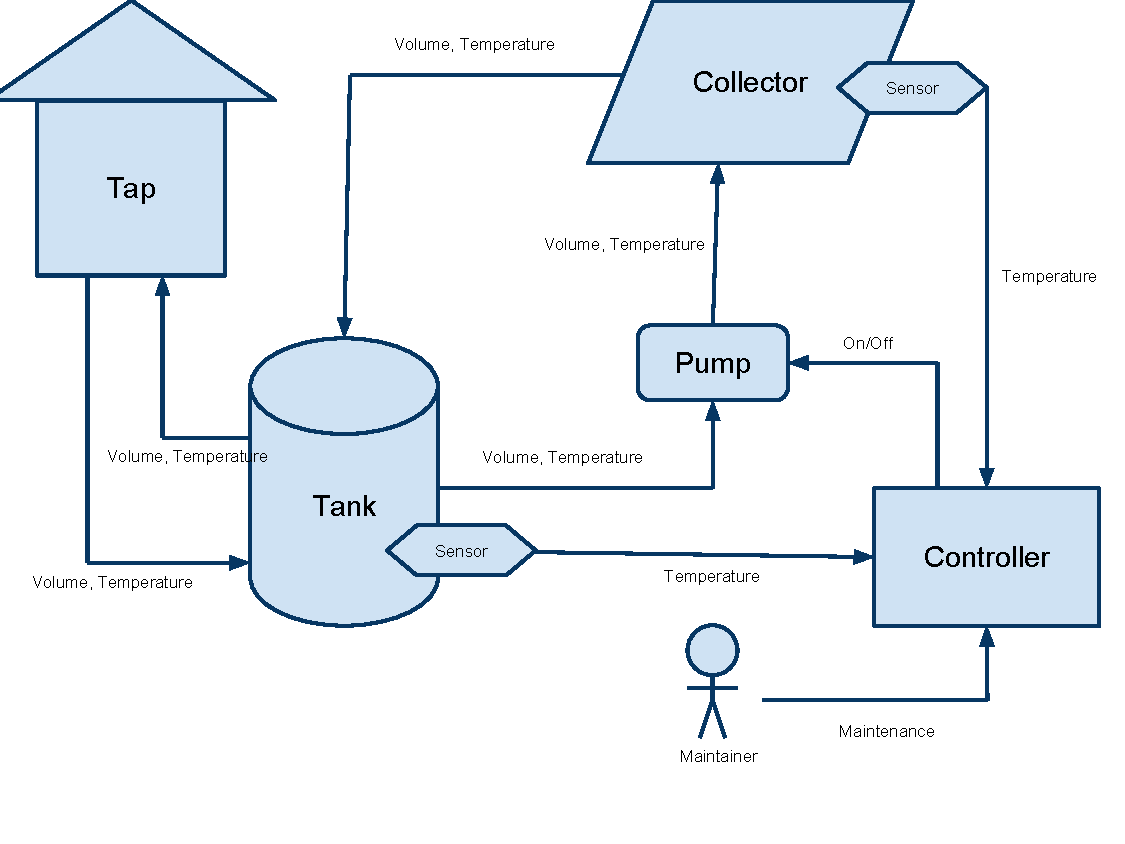
\includegraphics[scale=0.8]{schema.pdf}
\caption{System schematics}
\end{figure} 


The system consists of the following components:

\begin{itemize}

\item Water tank

\item Solar collector

\item Pump

\item Tap

\item Temperature sensors

\item Controller

\item Maintenance service

\end{itemize}

The hydraulic part of the system is modeled in terms of water containers (of which the tank and the collector are subclasses) and pumps (of which the tap is treated as a subclass) that drive the flow of water between containers. The connection between pairs of hydraulic components is treated as unidirectional (the presence of valves is implied) and consists of two variables representing the volume of water flowing from the source to the sink container over a time unit, and the temperature of the water. Water containers have an intrinsic volume, and have at least one input and one output port (each consisting of paired volume/temperature variables), but may have more. Heat transfer happens by water flow (which each container adjusting the temperature of the water within according to the inflow and outflow) and by absorption (or, in principle, dissipation) of heat within a container; the tubing is treated as perfectly insulated and leak-proof.

The connections between water containers and sensors represent the physical interaction with the sensor's thermometer. All connections involving the controller represent electronic signals, except for the connection to the maintainer component, which could be physically realized as a switch that the maintenance operator turns on while he's working on the system.

\setmonofont[Scale=0.8]{Menlo}

\pagebreak
\begin{adjustwidth}{-4em}{-4em}
\VerbatimInput[frame=lines, obeytabs=true, tabsize=2, label=\fbox{heatingsystem.trio},framesep=4mm]{../models/heatingsystem.trio}
\end{adjustwidth}
\pagebreak

\section{Controller}

The controller is the main component implementing the "intelligence" of the system. As such, while the axioms in most other components are a description of (and follow from) the physical behavior of those components, in the controller the axioms represent the requirements for the development of the appropriate control software.

The controller samples the temperature of the water in the tank and in the collector via Sensor components, and controls the Pump component. When the temperature difference is high enough, the pump is turned on; when it is low enough, it is turned off. Hysteresis ensures that the system does not keep flicking on and off around a boundary. The controller also takes care to turn the pump off during maintenance.

Note that we assume that the pump is either on or off, and switches between the two states "instantaneously" (that is, within a system tick). If the pump had a slow transition, the controller would need to be changed accordingly.

\pagebreak
\begin{adjustwidth}{-4em}{-4em}
\VerbatimInput[frame=lines, obeytabs=true, tabsize=2, label=\fbox{controller.trio},framesep=4mm]{../models/controller.trio}
\end{adjustwidth}
\pagebreak

\section{Sensor}

The sensor component models the sampling of temperature data. The thermometer variable is connected to a temperature variable on a physical component, and thus tracks the temperature at each time instant. The temp\_reading variable is connected to the controller, and holds the value that the thermometer input had at the last sampling instant.

Note that, physically, this memory would be located in the controller, but by modeling it inside the Sensor class we can connect as many sensors as needed without having to add memory variables to the controller class.

Furthermore, this class also models the controller's sampling timing, by means of a simple constant. If there were more classes that depended on this timing clock, it would make sense to move it into a separate clock component connected to all of the interested clients.

\pagebreak
\begin{adjustwidth}{-4em}{-4em}
\VerbatimInput[frame=lines, obeytabs=true, tabsize=2, label=\fbox{sensor.trio},framesep=4mm]{../models/sensor.trio}
\end{adjustwidth}
\pagebreak

\section{Water container}

The water container class describes a volume of water at a certain temperature with the ability to add or remove water from it. A water container knows how to mix the water it holds with a given volume of water at a given temperature.

All water containers have a constant volume. One may drain water out of a container, but it must be concurrently replaced by an equal volume. This is captured in the volume\_remains\_constant axiom.

By default water comes from one pipe and drains out of another, but the WaterContainer class is structured so that additional pipes can be attached. This is done through the definition of the axioms delta\_volume\_definition, total\_out\_volume\_definition (the net amount of volume coming out of the container), and total\_in\_volume\_temperature\_product\_definition (the sum of the products of each volume coming in and its corresponding temperature). Any subclasses that consider inputs and outputs from extra pipes can redefine these accordingly in order to retain the core functionality of a WaterContainer.

The following equations capture how temperature and volume change in a water container.

\subsection{Volume}

\begin{eqnarray*}
V_1 &=& V_0 + \Delta V\\
\Delta V &=& V_{in} - V_{out}
\end{eqnarray*}

$\Delta V$ is captured in the delta\_volume\_definition axiom to allow for further extension as we'll see later.

\subsection{Temperature}

At each time step, some water flows out of the container (at the temperature the container had at that point), and new water flows in; the final temperature of the container results from the mixing of the incoming water with the water left in the container. On top of this, the temperature can also be changed by heat exchange with external sources.

\begin{eqnarray*}
T_1 &=& \dfrac{(V_0 - \sum{V_{out_{i}}})T_0 + \sum{V_{in_{i}} T_{in_{i}}}}{V_1} + \dfrac{\Delta Q}{c \rho V_1}\\
&=& \dfrac{V_{0} T_0 + \alpha - \beta}{V_1} + \dfrac{\Delta Q}{c \rho V_{1}}\\
\alpha &=& \sum{V_{in_{i}}T_{in_{i}}}\\
\beta &=& \sum{V_{out_{i}}T_0} = V_{out-total}T_{0}
\end{eqnarray*}

Where $c$ and $\rho$ are the specific heat and density of water respectively. Note that these formulas only reflect reality if the water is always in a liquid state.

By default we assume a water container to have no heat loss or gain due to external sources. Therefore, in a standard water container we know:

\begin{eqnarray*}
\Delta Q = 0
\end{eqnarray*}

This is captured in the delta\_heat\_definition axiom. 

Furthermore, the standard water container has only one input port and one output port, so the definitions of $\alpha$ and $V_{out-total}$ involve a single volume and temperature each:

\begin{eqnarray*}
\alpha &=& V_{in}T_{in}\\
V_{out-total} &=& V_{out}
\end{eqnarray*}

\pagebreak
\begin{adjustwidth}{-4em}{-4em}
\VerbatimInput[frame=lines, obeytabs=true, tabsize=2, label=\fbox{water\_container.trio},framesep=4mm]{../models/water_container.trio}
\end{adjustwidth}
\pagebreak

\section{Collector}


The collector is the element that transfers heat from the sun into whatever volume of water it's currently holding. It is in essence a regular WaterContainer, which receives additional heat from an external source. Therefore, the same equations as for the base WaterContainer apply, except that we need to take into account the heat input from the sun by:

\begin{eqnarray*}
\Delta Q = Q_{sun}
\end{eqnarray*}

In order to achieve that all the Collector has to do is to redefine the delta\_heat\_definition in a manner consistent with the above equation.

\pagebreak
\begin{adjustwidth}{-4em}{-4em}
\VerbatimInput[frame=lines, obeytabs=true, tabsize=2, label=\fbox{collector.trio},framesep=4mm]{../models/collector.trio}
\end{adjustwidth}
\pagebreak

\section{Tank}

The tank is the main reservoir of hot water which our users will be using. It is in essence a WaterContainer, but with two extra pipes. The basic WaterContainer already has two pipes, which allows us to connect the tank to the collector, but it also needs a pipe taking hot water to the user, and another taking cold water from the aqueduct to replenish it: both of these ports are connected to a Tap instance.

The user uses water from the tank through the tap\_out\_volume and tap\_out\_temperature variables. As a condition of any water container, any water used must be instantly replaced by an equal volume, which the Tap ensures through tap\_in\_volume and tap\_in\_temperature. Once those are in place, the way the volume and temperature in the tank change is only slightly more complicated than a basic WaterContainer. The main equation is the same, but we need to redefine $\alpha$ and $V_{out-total}$ to take into account the four ports:

\begin{eqnarray*}
\alpha &=& V_{in}T_{in} + V_{in-tap} T_{in-tap}\\
 V_{out-total} &=& V_{out} + V_{out-tap}
\end{eqnarray*}

This is achieved by redefining the total\_in\_volume\_temperature\_product\_definition and total\_out\_volume\_definition axioms to reflect the fore-mentioned quantities ($\alpha$ and $V_{out-total}$ respectively).

As for the volume, the only difference compared to a default water container is that $\Delta V$ needs to consider the volumes coming in and out of the tap (consumption by the user, and corresponding resupply). 

\begin{eqnarray*}
\Delta V =  V_{in} + V_{in-tap} - V_{out} - V_{out-tap}
\end{eqnarray*}

Therefore, the Tank needs to redefine the delta\_volume\_definition axiom to reflect that.

\pagebreak
\begin{adjustwidth}{-4em}{-4em}
\VerbatimInput[frame=lines, obeytabs=true, tabsize=2, label=\fbox{tank.trio},framesep=4mm]{../models/tank.trio}
\end{adjustwidth}
\pagebreak

\section{Pump}

The pump is a class which describes the behaviour of the active hydraulic part of the system. As the name suggests, the pump is responsible for moving the water from one of its sides to the others. Considering the actual complexity of a real-world application, a few assumptions have been made so that the formal description becomes easier. Control and state are predicates which describe when the pump is started and stopped, and when the pump is operational and when it isn't, respectively. Both of the predicates are visible as they are connected to the equivalent predicates of the controller class. The four variables describe the volume and temperature of the water entering and exiting the pump respectively, in a given time unit. We assume that the temperature increase in the water due to the pump's operation is negligible, therefore the temperature of the water flowing out is the same as that of the water flowing in. The constant value pump\_volume is used to describe a property of the pump, that is the volume of water moved per time unit when in operation. As shown by the predicate state, the pump can either be on or off.

The following properties are stated through the use of axioms. To begin with, the amount of water getting into the pump has to be the same of the volume of water getting out of it. This is because the water cannot create new water and at the same time there are no water leaks. As stated above, the entering temperature is considered as the same of the exiting one. This is unquestionably a simplification, but the effects shouldn't change the accuracy of the model significantly, as in a real-life application extra care would be taken to isolate all tubes as much as possible. The following two axioms describe the behaviour of the water subject to the pump state: if the pump is off for a given time unit, then the moved volume is 0; on the other hand if the pump is on the volume of the moved water is pump\_volume, which is the maximum amount of water the pump can move in a time unit. The start and stop axioms make sure that, after receiving a control signal, the pump keeps the required state (on or off) until it receives the opposite signal. Finally, since states of the pump are described with state(on) and state(off) which can each be true or false, there is an axiom which states that the pump cannot be in an active state while being off and vice-versa.

\pagebreak
\begin{adjustwidth}{-4em}{-4em}
\VerbatimInput[frame=lines, obeytabs=true, tabsize=2, label=\fbox{pump.trio},framesep=4mm]{../models/pump.trio}
\end{adjustwidth}
\pagebreak

\section{Tap}

The tap is a pretty simple class which models the behaviour of the final users of warm water. Since this use of water can be seen as a replacement of hot water taken from the tank with cold water from the pipes supply, this is described starting from the class pump. There is a very significant difference between the two, which can be solved by re-writing the rule for the axiom SameTemp. In fact in the pump there is no temperature difference between water in and out, while with the tap there is. What needs to be connected here is the temperature of the water going into the tank from the pipes supply with the variable describing it. The variable cold\_supply\_temperature is visible as this is an external parameter that, in a real system, would change mainly based on the season but also on some minor aspects and for this very reason it is visible in the heating\_system overall.

\pagebreak
\begin{adjustwidth}{-4em}{-4em}
\VerbatimInput[frame=lines, obeytabs=true, tabsize=2, label=\fbox{tap.trio},framesep=4mm]{../models/tap.trio}
\end{adjustwidth}
\pagebreak

\section{Maintainer}

The class maintainer describes the person who is responsible for the maintenance of the collector. This has to be performed once per year. The fact that it might not be possible to perform the maintenance exactly one year after the previous check has been taken into account by replacing the exact one-year period with a time window. Any time in that time frame would be acceptable. There are two predicates: the first one, which is called startwork, indicates when the maintainer starts performing the check. This is visible because it is external in the real world: this depends on when the maintainer actually comes to work on the collector. The second one is called working and is true when the maintainer is working on the collector. The reason why this second one is visible is that it has to be connected to the controller of the system. In fact, when the maintainer is working the system should be in a maintenance state which would stop the pump for the entire time of the procedure. Actually this is sufficient to describe all effects the check has: in the end the volumes won't be changed, and during the procedure the collector won't be able to raise the temperature of the water going to the tank, because all water going to the tank would come from the pipes. In terms of axioms the following properties must be granted: the maintenance procedure has to be undertaken no more than once every min\_maintenance\_interval, but no less that once every max\_maintenance\_interval. It is also true that in the beginning the maintainer isn't working: in fact if s/he never started, then at a given time s/he isn't working. Moreover the maintainer should be working for a time represented by the constant worktime after starting work. Finally the maintainer should stop working after a time worktime and s/he shouldn't work until the predicate startwork becomes true again.

\pagebreak
\begin{adjustwidth}{-4em}{-4em}
\VerbatimInput[frame=lines, obeytabs=true, tabsize=2, label=\fbox{maintainer.trio},framesep=4mm]{../models/maintainer.trio}
\end{adjustwidth}
\pagebreak

\section{Possible improvements}

In terms of physical modeling, the main simplifications adopted are the use of a time-discrete model and the assumption of a uniform temperature within each water container. The former seems unavoidable: an accurate time-continuous model would require the use of integrals and derivatives, which are not available in TRIO. None of us is a hydraulic engineer, but we would not be surprised if it turned out that a thoroughly accurate physical model did not have a closed form solution anyway, and would require numerical integration.

The assumption of a uniform temperature within containers is perhaps a more significant simplification, especially when timing is considered. One could picture the time-discrete approximation as replacing a constant flow of water through the pipes with pouring volumes of water with buckets at regular intervals: on one hand, the system period must be sufficiently small for this time-discrete approximation to approximate a continuous flow; on the other hand, it needs to be sufficiently large for temperature differences to even out. We could abandon the uniform temperature simplification by breaking up the water containers (especially the tank) into several smaller volumes of water, and modeling diffusion and convection as the interactions between them; it may be sufficient to have two parts for the tank to represent a temperature gradient between hotter water at the top and colder water at the bottom. On the other hand, increasing the complexity of the system would slow down the verification process, so we chose to keep things simple.

\end{document}